% InsightFlow AI: An Inspectable, Confidence-Aware Pipeline for Conversational Business Intelligence
% Conference-format draft (IEEEtran, conference mode). Target venue not yet confirmed:
% this draft does not claim compliance with any specific conference's rules.
% TO DO before submission:
%   1. Replace every red \authorcheck{...}: four e-mail addresses and the corresponding author.
%   2. Confirm author names and affiliations; confirm venue template, page limit, paper size
%      (add a4paper to \documentclass if the venue requires A4) and disclosure requirements.
%   3. Figures: figures/fig_*.pdf are built from figures/src/*.tex (see figures/README.txt).
%   4. Reference [3]: add the track designation only if confirmed; reference [8]: add an access
%      date and, if MCP stays in the paper, the specification revision actually implemented.
%   5. Round 7 revision (this file): Fig. 5 (figures/fig_r7_ablation.pdf) was rendered with matplotlib
%      because no TeX installation was available; rebuild it from figures/src/fig_r7_ablation.tex to match
%      the other figures if preferred. This file was NOT compiled after the Round 7 edits; compile and check
%      layout, float placement and page count against the venue limit.
%   6. The Round 7 artifacts (revision 38b60d1 and later) were committed locally; push them before citing
%      the repository as containing them.
%   8. Round 8 revision (this file): adds Section IV-G/V-K..V-M; not compiled; check page count.
%   7. AI-assistance disclosure: the Round 7 implementation changes, question set and these edits were
%      produced with an AI coding agent. Check the venue's policy and add the required statement.
\documentclass[conference]{IEEEtran}
\usepackage{cite}
\usepackage{amsmath,amssymb}
\usepackage{booktabs}
\usepackage{graphicx}
\usepackage{array}
\usepackage{url}
\usepackage{xcolor}
\providecommand{\tightlist}{\setlength{\itemsep}{0pt}\setlength{\parskip}{0pt}}
\newcommand{\authorcheck}[1]{\textcolor{red}{#1}}

\begin{document}

\title{InsightFlow AI: An Inspectable, Confidence-Aware Pipeline for Conversational Business Intelligence}

\author{%
\IEEEauthorblockN{Kethemreddy Jagankumarreddy}
\IEEEauthorblockA{\textit{School of Computer Science and Engineering}\\
\textit{Vellore Institute of Technology}\\
Vellore, Tamil Nadu, India -- 632014\\
\authorcheck{[email 1]}}
\and
\IEEEauthorblockN{Smitha Kattuboina}
\IEEEauthorblockA{\textit{School of Computer Science and Engineering}\\
\textit{Vellore Institute of Technology}\\
Vellore, Tamil Nadu, India -- 632014\\
\authorcheck{[email 2]}}
\and
\IEEEauthorblockN{Nimmakayala Akshya}
\IEEEauthorblockA{\textit{School of Computer Science and Engineering}\\
\textit{Vellore Institute of Technology}\\
Vellore, Tamil Nadu, India -- 632014\\
\authorcheck{[email 3]}}
\and
\IEEEauthorblockN{Madhu Vishanadan}
\IEEEauthorblockA{\textit{School of Computer Science and Engineering}\\
\textit{Vellore Institute of Technology}\\
Vellore, Tamil Nadu, India -- 632014\\
\authorcheck{[email 4]}\\
Corresponding author: \authorcheck{[to be confirmed]}}
}

\maketitle

\begin{abstract}
Conversational business intelligence systems translate natural-language questions into database queries, but syntactically valid queries can still fail to preserve the user's intended analytical meaning. This paper presents InsightFlow AI, an inspectable pipeline that combines query planning, confidence-aware response selection, evidence recording, and a semantic correctness layer. The semantic layer checks whether requested measures, filters, grouping, temporal interpretation, join paths, and output structure are preserved through query execution and response generation. The system supports four response actions: answer, warn, clarify, and abstain.

We report three experiments that are not pooled. In a historical 27-question benchmark on a synthetic sales database, an earlier pipeline agreed with reference SQL on 15 of 17 answerable questions. In a sealed 66-question first run over airline, software-as-a-service (SaaS), and farm schemas (K1), the semantic-layer implementation answered 42 of 54 answerable questions correctly and produced two silent wrong answers, both with internal confidence near 0.98. In a third evaluation (R7), a later revision was frozen and run once on 105 new questions over four synthetic schemas authored by a separate agent process; these questions are not human-adjudicated. The system answered 14 of 74 answerable questions correctly (18.9\%), left 57 unanswered, declined 27 of 31 questions that required clarification or were out of scope, and gave 7 wrong answers among the 105 questions. With six post-generation safeguards disabled, the same build gave 32 wrong answers and 17 correct ones. Paired ablations attribute most of this reduction to checks that compare the question's wording with the executed query, and part to the semantic layer; four other safeguards changed no outcome. Every R7 answer, correct or not, had confidence of at least 0.979. After inspecting the R7 failures we revised the planner's grounding; on the revealed R7 questions the revised build answers 63 of 74 correctly (post-hoc, not held out), but on a further blind set of 106 questions over four new schemas (R8) it answered only 5 of 73 answerable questions correctly and gave 10 wrong answers, so the improvement did not generalize. On R8 the internal confidence score did not separate correct from wrong answers (AUROC 0.45).

The results show that explicit checks of the question against the executed query can prevent most silent errors on unfamiliar schemas, at a large cost in coverage, and that the internal confidence score is not calibrated. The experiments do not establish general superiority over existing systems or elimination of semantic errors.
\end{abstract}

\begin{IEEEkeywords}
Conversational business intelligence, text-to-SQL, semantic validation, explainable analytics, confidence-aware systems, selective prediction, query verification, ablation study
\end{IEEEkeywords}

\section{Introduction}

Business intelligence systems help organizations examine operational data, monitor performance indicators, and investigate changes in business activity. Traditional interfaces often require users to understand database schemas, query languages, or predefined dashboards. Natural-language interfaces offer an alternative by allowing users to express analytical questions in familiar terms.

However, translating a natural-language question into SQL involves more than generating a query that executes successfully. The generated query must preserve the intended measure, filtering conditions, grouping level, temporal interpretation, relationships between tables, and expected output structure. A query can be syntactically valid and return plausible values while still answering a different question from the one the user asked.

For example, a request to calculate revenue excluding cancelled orders can be misinterpreted as a request to calculate revenue from cancelled orders. A request for yield per acre may produce separate totals for yield and acreage rather than a ratio. A query involving multiple tables may duplicate records if the join relationships or aggregation grain are handled incorrectly. These failures are difficult to detect through syntax validation alone because the database can execute the query without raising an error.

Research on natural-language-to-SQL systems has advanced substantially through datasets and benchmarks such as Spider, BIRD, and Spider 2.0 \cite{yu2018spider,li2023bird,lei2025spider2}. These resources provide increasingly demanding settings for evaluating semantic parsing, database grounding, and query execution. Nevertheless, the success of an individual query execution does not by itself establish that the resulting answer matches the user's intended analytical meaning.

InsightFlow AI is a prototype designed to investigate how conversational business intelligence can combine query planning with inspectable evidence, confidence-aware response selection, and explicit semantic checks. The system records relevant information about the request, the generated SQL, the applied filters, and the resulting data. It also supports four response actions: ANSWER, WARN, CLARIFY, and ABSTAIN. The intention is to make the system's decision and supporting evidence easier to inspect while allowing unresolved or potentially unsafe requests to be handled conservatively.

A central design consideration is the distinction between confidence and correctness. An internal confidence score can summarize the signals available to a system, but a high score does not establish that a query preserves the user's intended meaning. Accordingly, InsightFlow AI includes a semantic correctness layer that checks selected aspects of the analytical request before and after query execution. The checks cover supported properties such as measure compatibility, filter polarity, grouping, temporal constraints, join paths, and output shape.

This paper evaluates the prototype through three separate experiments. The first is a historical benchmark of an earlier pipeline on a synthetic sales database. The second evaluates the first-run behaviour of the semantic-layer implementation on a sealed set of questions spanning three database schemas (Round 6). The third freezes a later revision and runs it once on 105 new questions over four further schemas written by a separate agent process (Round 7), and then disables the safeguards one at a time on the same build. A fourth step revises the implementation using the R7 failures and evaluates the revised, frozen build on a new blind set (Round 8). The results are reported separately because the experiments use different system revisions, datasets, and evaluation protocols.

The contributions of this paper are as follows:

\begin{enumerate}
\def\labelenumi{\arabic{enumi}.}
\item
  \textbf{Inspectable pipeline design:} We describe a conversational business intelligence pipeline combining query planning, database execution, semantic checks, evidence recording, and confidence-aware response selection.
\item
  \textbf{Three-stage empirical evaluation:} We report historical reference-SQL agreement results, a sealed first-run evaluation of semantic validation across airline, SaaS, and farm schemas, and a frozen first run on four new schemas whose questions were written without access to the implementation.
\item
  \textbf{Safeguard ablation:} On the frozen Round 7 build we disable each post-generation safeguard alone, all together, and all but one, and attribute each prevented error to a component through paired per-question transitions.
\item
  \textbf{Failure-oriented analysis:} We document examples of incorrect high-confidence answers, unresolved answerable questions, and limitations in the current semantic checks. We distinguish initial results from improvements measured after the failure cases had been inspected.
\end{enumerate}

The paper does not claim that InsightFlow AI outperforms established text-to-SQL systems. Instead, it presents a bounded evaluation of the current prototype, with emphasis on inspectability, semantic failure detection, and the relationship between answer coverage and incorrect responses.

\section{Related Work}

\subsection{Natural-Language-to-SQL Systems}

Seq2SQL explored the generation of structured queries from natural-language questions using reinforcement learning \cite{zhong2017seq2sql}. Spider introduced a large, cross-domain benchmark requiring models to generate SQL for databases that may not have appeared during training \cite{yu2018spider}. BIRD expanded the evaluation setting through large databases and challenges involving value grounding and real-world database content \cite{li2023bird}. Spider 2.0 considers more complex enterprise workflows and database environments \cite{lei2025spider2}.

These studies provide important foundations for evaluating natural-language-to-SQL capabilities. InsightFlow AI addresses a complementary system-level concern: after a candidate query has been constructed, how can the system inspect whether the query preserves the intended analytical request?

The present evaluation is not a direct comparison with these benchmarks. It uses project-specific synthetic datasets and does not establish comparative performance against the systems evaluated in the cited work.

\subsection{Selective Prediction and Abstention}

Selective prediction studies systems that may decline to make a prediction when the available evidence is insufficient. This creates a trade-off between coverage, which measures how often a system responds, and the risk of error among the responses it provides \cite{geifman2017selective}.

The same trade-off arises in conversational business intelligence. A system that asks for clarification on every difficult request may avoid some incorrect answers but provide limited analytical coverage. A system that answers aggressively may be more responsive while producing plausible but incorrect results.

InsightFlow AI implements response actions intended to distinguish direct answers from warnings, clarification requests, and abstentions. Its evaluation therefore considers both correctness and the handling of questions that should not be answered directly.

\subsection{Confidence Estimation and Calibration}

Confidence estimates can support decisions about whether to answer or request clarification. However, confidence is useful only when its relationship with observed correctness is understood.

Expected calibration error (ECE) is one commonly used summary of calibration. It compares average confidence with empirical accuracy across confidence bins \cite{naeini2015bbq}. Its interpretation depends on the population, binning strategy, and definition of correctness.

The earlier InsightFlow AI pipeline combines several internal signals into a composite confidence score. The newer semantic-layer evaluation examines whether high scores correspond to correct outputs. The results show why confidence, correctness, coverage, and silent error counts must be reported separately rather than treating a confidence value as a guarantee.

\subsection{Evidence and Tool-Oriented Systems}

ReAct combines reasoning and action in language-model-based systems \cite{yao2023react}. The Model Context Protocol (MCP) defines a standard interface through which applications can expose tools and contextual information to clients \cite{mcp}.

InsightFlow AI includes evidence-recording capabilities and tool-server integration in its broader implementation. However, the experiments reported in this paper do not evaluate MCP interoperability or compare tool-use frameworks. Evidence visibility is treated as an inspectability feature, not as proof that the generated query is correct.

Table~\ref{tab:related} summarizes the cited work and its role in this paper.

\begin{table}[!t]
\caption{Related Work and Its Role in This Paper}
\label{tab:related}
\centering
\footnotesize
\setlength{\tabcolsep}{3pt}
\begin{tabular}{@{}>{\raggedright}p{0.25\columnwidth}>{\raggedright}p{0.39\columnwidth}>{\raggedright\arraybackslash}p{0.30\columnwidth}@{}}
\toprule
\textbf{Work} & \textbf{Contribution and focus} & \textbf{Role in this paper} \\
\midrule
Seq2SQL \cite{zhong2017seq2sql} & Method: natural-language-to-SQL generation with reinforcement learning & Background; not compared \\
Spider \cite{yu2018spider} & Benchmark: cross-domain text-to-SQL & Background; not evaluated on \\
BIRD \cite{li2023bird} & Benchmark: large-scale, database-grounded text-to-SQL with external knowledge & Background; not evaluated on \\
Spider 2.0 \cite{lei2025spider2} & Benchmark: enterprise text-to-SQL workflows & Background; not evaluated on \\
Selective classification \cite{geifman2017selective} & Method: abstention under a risk--coverage trade-off & Motivates the answer/clarify trade-off \\
Bayesian binning \cite{naeini2015bbq} & Method: calibration; expected calibration error & ECE used as a diagnostic \\
ReAct \cite{yao2023react} & Method: interleaved reasoning and tool actions & Context; not evaluated \\
MCP \cite{mcp} & Protocol: exposing tools and context to applications & Servers implemented; not evaluated \\
InsightFlow AI (this work) & Prototype: typed plan, semantic checks, four actions, evidence record & Evaluated on synthetic SQLite schemas only \\
\bottomrule
\end{tabular}

\vspace{3pt}
\parbox{\columnwidth}{\scriptsize Comparison of scope and role only; no system was compared experimentally.}
\end{table}


\section{System Design}

\subsection{Architecture Overview}

InsightFlow AI is implemented as a web-based conversational business intelligence prototype. The frontend uses Next.js 14.2.5, while the backend uses Python FastAPI and SQLAlchemy for database access. SQLite is the default database used in the reported experiments. PostgreSQL connectivity has not been evaluated as part of the reported results.

The default planner is deterministic and rule-based. An optional language-model client exists in the broader implementation, but it was disabled in the reported runs. Consequently, the results should not be interpreted as an evaluation of an LLM-driven query planner.

The pipeline can be summarized in the following stages:

\begin{enumerate}
\def\labelenumi{\arabic{enumi}.}
\tightlist
\item
  Receive the natural-language question and available database context.
\item
  Identify the analytical intent and construct a candidate plan.
\item
  Resolve relevant schema elements and candidate measures.
\item
  Construct a candidate SQL query.
\item
  Apply query and execution-safety checks.
\item
  Execute the query against the selected database.
\item
  Check selected semantic properties against the request and result.
\item
  Assemble the supporting evidence record.
\item
  Select a response action and present the result, warning, clarification request, or abstention.
\end{enumerate}

The stages provide inspection points for diagnosing failures. The pipeline does not assume that successful execution is sufficient to establish correctness.

Fig.~\ref{fig:arch} shows these components and the data flow. The evaluation harness calls the orchestrator directly, so the web frontend, the REST API and the MCP tool servers were not exercised by the reported experiments.

\begin{figure*}[!t]
\centering
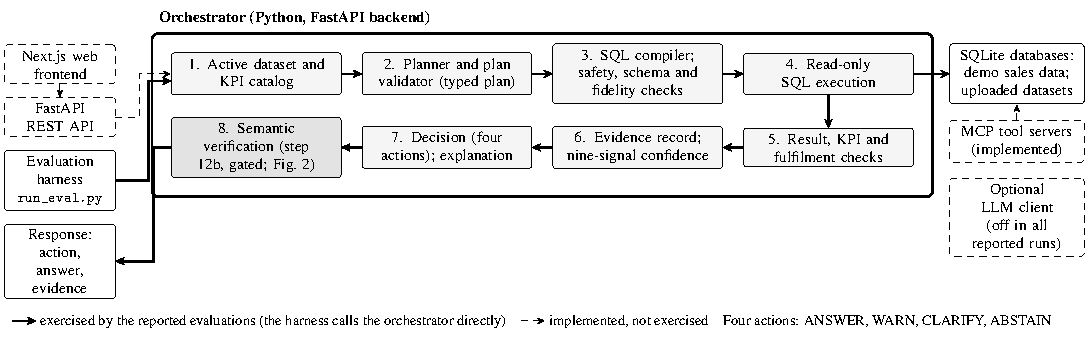
\includegraphics[width=\textwidth]{figures/fig_architecture.pdf}
\caption{System architecture of InsightFlow AI, derived from the orchestrator pipeline; the stages shown are present at revisions \texttt{78d906b} (K1), \texttt{a63cec1} (K3), \texttt{b11793b} and \texttt{38b60d1} (R7). Solid arrows mark paths exercised by the reported evaluations, whose harness calls the orchestrator directly; dashed elements are implemented but were not exercised. The semantic verification stage applies only under the conditions shown in Fig.~\ref{fig:semflow}.}
\label{fig:arch}
\end{figure*}


\subsection{Response Actions}

The system supports four response actions.

\textbf{ANSWER:} The system returns a result when the applicable checks do not identify a blocking issue.

\textbf{WARN:} The system returns a result with a caveat or stated assumption when an issue has been identified but does not trigger a complete block.

\textbf{CLARIFY:} The system requests additional information when the analytical intent or necessary schema interpretation cannot be resolved sufficiently.

\textbf{ABSTAIN:} The system declines to produce a direct answer when the request falls outside supported capabilities or cannot be handled within the current constraints.

These actions are intended to make uncertainty operationally visible. They do not imply that every incorrect query will be detected or that every request requiring clarification will be identified correctly.

\subsection{Confidence-Aware Decision Signal}

The earlier pipeline computes a composite confidence score from nine signals:

\begin{itemize}
\tightlist
\item
  SQL validity;
\item
  schema match;
\item
  KPI match;
\item
  context consistency;
\item
  data completeness;
\item
  evidence strength;
\item
  result consistency;
\item
  intent coverage; and
\item
  plan fidelity.
\end{itemize}

The associated weights are 0.12, 0.10, 0.13, 0.13, 0.08, 0.07, 0.10, 0.13, and 0.14, respectively. These weights sum to 1.00.

The historical implementation used a high threshold of 0.70 and a low threshold of 0.40. It also capped the composite score using intent coverage and plan fidelity:

\begin{equation}
C = \min\bigl(S,\ \mathrm{coverage}+0.05,\ \mathrm{fidelity}+0.05\bigr),
\label{eq:cap}
\end{equation}

where \(S\) is the weighted signal score.

The score is an internal decision signal, not a statistically calibrated probability that an answer is correct. The first-run semantic-layer evaluation includes high-confidence incorrect outputs, which demonstrates the importance of evaluating confidence against observed outcomes.

\subsection{Semantic Correctness Layer}

The newer implementation adds a semantic validation package containing a semantic specification, type checks that compare the specification with the wording of the question, preservation checks against the executed SQL, the result rows and the written answer, and a verifier that returns findings classified as violations or notes. The package runs after execution, as step 12b of the pipeline (Fig.~\ref{fig:semflow}); the type checks do not use the executed SQL or rows.

The layer checks selected properties of a request and its execution plan, including:

\begin{enumerate}
\def\labelenumi{\arabic{enumi}.}
\item
  \textbf{Measure compatibility:} Whether the requested measure is compatible with the type and meaning of the referenced column.
\item
  \textbf{Filter preservation:} Whether exclusions, negation, and filter polarity are preserved in the generated query.
\item
  \textbf{Aggregation and output shape:} Whether the query produces the expected scalar or grouped result structure.
\item
  \textbf{Temporal interpretation:} Whether date constraints and the selected date column are consistent with the request.
\item
  \textbf{Join grounding:} Whether the join path is supported by available schema relationships and whether the join may multiply records.
\item
  \textbf{Ratio handling:} Whether a request for a ratio is represented by a ratio calculation rather than separate totals. This check was added after the K1 run, in response to case V07; it is part of the K3 configuration but was not present at revision \texttt{78d906b}.
\item
  \textbf{Result and explanation consistency:} Whether numerical claims in the explanation correspond to the query result and whether the result structure matches the request.
\end{enumerate}

A detected violation changes a pending ANSWER or WARN to CLARIFY and caps the confidence at 0.30. Findings of severity note are recorded in the response diagnostics and do not change the action. The layer runs only when the pending action is ANSWER or WARN, the dataset is not the built-in demo dataset, SQL was executed successfully, and the plan has one of the intent kinds direct KPI, breakdown, top-$N$ or trend; the planner's \texttt{ratio} intent kind (``X per Y over KPIs) was added in revision \texttt{a63cec1}. Other intents and the demo dataset are not checked by this layer. Table~\ref{tab:rules} lists the implemented rules. If the verifier itself raised an exception, revisions \texttt{78d906b} and \texttt{a63cec1} logged the error and left the decision unchanged (fail-open); revision \texttt{b11793b}, committed after both Round 6 runs, returns CLARIFY instead (fail-closed). No Round 6 results are reported for that revision. The Round 7 evaluation (Section~\ref{sec:r7method}) uses revision \texttt{38b60d1}, which includes the fail-closed handling and one further rule, \texttt{count\_\allowbreak{}of\_\allowbreak{}measure\_\allowbreak{}noun}.

The semantic layer is rule-based and only covers selected classes of errors. It does not formally prove equivalence between the user's intended question and the generated SQL. Unrecognized wording, incomplete schema information, unsupported analytical patterns, or limitations in the rules may still result in an incorrect response.


\begin{figure}[!t]
\centering
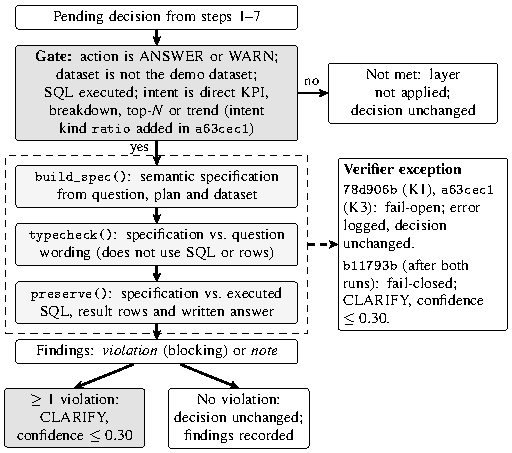
\includegraphics[width=\columnwidth]{figures/fig_semantic_workflow.pdf}
\caption{Semantic-layer workflow (step 12b). The gate restricts verification to non-demo datasets, executed SQL and the listed intent kinds. A violation turns a pending answer into CLARIFY with confidence at most 0.30. Verifier exceptions were handled fail-open at the K1 and K3 revisions and fail-closed from \texttt{b11793b}, after both runs.}
\label{fig:semflow}
\end{figure}

\begin{table}[!t]
\caption{Implemented Semantic Rules at Revision 38b60d1}
\label{tab:rules}
\centering
\footnotesize
\setlength{\tabcolsep}{2.5pt}
\begin{tabular}{@{}>{\raggedright}p{0.42\columnwidth}>{\raggedright}p{0.43\columnwidth}>{\centering\arraybackslash}p{0.085\columnwidth}@{}}
\toprule
\textbf{Rule codes} & \textbf{Detects} & \textbf{Since} \\
\midrule
\multicolumn{3}{@{}l}{\emph{Type checks: specification vs.\ question wording}} \\
\texttt{unresolved\_\allowbreak{}reference} & Unresolved part of the question when an answer was produced & K1 \\
\texttt{flag\_\allowbreak{}used\_\allowbreak{}as\_\allowbreak{}quantity}, \texttt{identifier\_\allowbreak{}used\_\allowbreak{}as\_\allowbreak{}quantity} & Aggregating a yes/no flag or an identifier as an amount & K1 \\
\texttt{entity\_\allowbreak{}count\_\allowbreak{}mismatch} & ``How many X'' answered by counting rows of another table & K1 \\
\texttt{shape\_\allowbreak{}scalar\_\allowbreak{}expected}, \texttt{shape\_\allowbreak{}breakdown\_\allowbreak{}expected}, \texttt{shape\_\allowbreak{}ranking\_\allowbreak{}expected} & Plan shape differs from the wording (single figure, breakdown, ranked list) & K1 \\
\texttt{date\_\allowbreak{}role\_\allowbreak{}guessed}, \texttt{date\_\allowbreak{}role\_\allowbreak{}mismatch} & Date column chosen without basis, or differing from the one named & K1 \\
\texttt{unsafe\_\allowbreak{}join}, \texttt{unsafe\_\allowbreak{}grouping\_\allowbreak{}path} & Join or grouping through a relationship that is not safely many-to-one & K1 \\
\texttt{polarity\_\allowbreak{}inverted} & Wording excludes a value that the query keeps & K3 \\
\texttt{ratio\_\allowbreak{}unsupported} & ``Per X'' ratio of two measures that the query does not compute & K3 \\
\texttt{count\_\allowbreak{}of\_\allowbreak{}measure\_\allowbreak{}noun} & ``How many X'' where X names a quantity column, answered by counting rows & R7 \\
\texttt{assumption} (note) & Recorded assumption; does not block & K1 \\
\multicolumn{3}{@{}l}{\emph{Preservation checks: executed SQL, rows and written answer}} \\
\texttt{measure\_\allowbreak{}not\_\allowbreak{}preserved} & Required aggregate missing from the SQL & K1 \\
\texttt{filter\_\allowbreak{}not\_\allowbreak{}preserved}, \texttt{exclusion\_\allowbreak{}not\_\allowbreak{}preserved} & Planned filter missing, or an exclusion lost its negation & K1 \\
\texttt{time\_\allowbreak{}not\_\allowbreak{}preserved} & Planned time bound missing & K1 \\
\texttt{grouping\_\allowbreak{}not\_\allowbreak{}preserved}, \texttt{ranking\_\allowbreak{}not\_\allowbreak{}preserved} & Dimension missing from GROUP BY; top-$N$ not applied & K1 \\
\texttt{unplanned\_\allowbreak{}join}, \texttt{fanout\_\allowbreak{}join} & Unneeded join, or one-to-many join that multiplies rows & K1 \\
\texttt{unexpected\_\allowbreak{}columns}, \texttt{shape\_\allowbreak{}violation} & Result columns or row count differ from the expected shape & K1 \\
\texttt{answer\_\allowbreak{}not\_\allowbreak{}faithful} & Written answer states a number absent from the result & K1 \\
\bottomrule
\end{tabular}

\vspace{3pt}
\parbox{\columnwidth}{\scriptsize All rules are blocking violations except \texttt{assumption}. K1: present at \texttt{78d906b}; K3: added in \texttt{a63cec1}, after the K1 run; R7: added in \texttt{38b60d1}, before the R7 run. Rules apply only under the gate conditions in Fig.~\ref{fig:semflow}.}
\end{table}

\subsection{Evidence Record}

The evidence record is intended to expose the information needed to inspect how an answer was produced. Depending on the execution path, it can include the original question, generated SQL, KPI definition, applied filters, calculations, result row count, and selected result rows.

This record can help distinguish failures in query execution from failures in interpreting the question. It also supports reproducibility and debugging by making the intermediate query and its result available for examination.

Evidence completeness and evidence correctness are separate properties. A record may contain a valid SQL statement and the values returned by the database while still documenting a query that applies the wrong filter or aggregation.

\subsection{Tool Integration}

The broader project includes tool-server integration intended to expose selected data and analysis operations through structured interfaces. The implementation inventory records multiple tool groups and server components. However, the experiments in this paper do not measure the reliability, interoperability, or performance of those integrations. They are therefore not treated as experimentally validated contributions in the reported results.

\section{Evaluation Methodology}

The evaluation comprises three experiments with different purposes. The historical benchmark measures an earlier pipeline on a synthetic sales database. The Round 6 evaluation measures the first-run behaviour of the newer semantic-layer implementation across three schemas. The Round 7 (R7) evaluation measures a later frozen revision on four new schemas and includes safeguard ablations. Results from these experiments are not pooled.

\subsection{Historical Sales Benchmark}

The historical benchmark uses a synthetic sales database containing:

\begin{itemize}
\tightlist
\item
  2,037 orders;
\item
  60 customers;
\item
  12 products;
\item
  four product categories;
\item
  four regions; and
\item
  records covering January through September 2026.
\end{itemize}

The synthetic data include a revenue decline in July for one region/category combination. The benchmark contains 27 author-written questions, classified as 17 answerable, four ambiguous, and six out of scope.

Five configurations were evaluated, producing 135 recorded runs in total. The historical results are tied to commit \texttt{3c843de88c\allowbreak{}a0b6266974\allowbreak{}9b217aaef0\allowbreak{}00e3e6363e}. They are not measurements of the later semantic-layer implementation.

The principal measures were SQL execution success, reference-SQL agreement, routing for non-answerable questions, question coverage, latency, and confidence calibration.

Reference-SQL agreement measures whether the generated query result agrees with the designated reference query under the benchmark's comparison procedure. It is not necessarily equivalent to independently adjudicated semantic correctness. If a reference query does not fully specify the intended analytical comparison, agreement or disagreement alone may be insufficient to determine whether the generated answer is semantically correct.

\subsection{Round 6 Semantic-Layer Evaluation}

The Round 6 evaluation contains 66 questions across three database schemas:

\begin{itemize}
\tightlist
\item
  airline data involving flights;
\item
  SaaS data involving invoices; and
\item
  farm data involving readings and harvests.
\end{itemize}

Reference results were prepared using independent SQLite SQL. The question set was sealed before the first run, and the implementation was frozen at commit \texttt{78d906b} before the sealed questions were inspected. This first-run configuration is identified as K1.

The evaluation includes answerable questions and questions expected to require clarification or otherwise not produce a direct answer. The recorded measures include:

\begin{itemize}
\tightlist
\item
  correct answers among answerable questions;
\item
  answered questions among answerable questions;
\item
  answerable questions left unanswered;
\item
  silent wrong answers among all questions;
\item
  correct clarification decisions; and
\item
  median and 95th-percentile latency.
\end{itemize}

A silent wrong answer is a returned answer classified as incorrect by the recorded evaluation reference, including cases where the expected outcome was clarification rather than a direct answer.

These measures have different denominators. In particular, the number of answerable questions answered should not be confused with the total number of answer outputs across all question classes. Results should be interpreted using the denominator specified for each metric.

\subsection{Post-Hoc Tuning Protocol}

After K1 was recorded, failure cases were inspected and implementation changes were made. The resulting K3 configuration was evaluated on the same set. Since the failure cases had already informed development, K3 is a post-hoc tuned result, not an independent held-out result.

K3 is included to document the observed effect of targeted fixes. K1 remains the primary first-run result for the sealed set. Neither result alone establishes generalization to unseen production databases.

\subsection{Round 7: Frozen First Run on Agent-Authored Schemas}
\label{sec:r7method}

After K3, development continued on the Round 6 schemas and on earlier development sets. The changes generalize patterns observed there: comparative wording (``larger than'', ``at least'') for numeric conditions on related tables, with an unrecognized comparative never read as equality; flags whose names state the normal condition (e.g.\ \texttt{sensor\_ok}) selected only when the question names that condition, its negation or a listed antonym such as ``faulty''; expanded abbreviations for measure names; a weaker foreign-key inference tier for role-prefixed text codes that share the key suffix of a single parent key and are fully contained in it, always disclosed with a warning; ``average X per'' the base-table row read as a plain average; semi-join filters for value-qualified fan-out phrases; and the rule \texttt{count\_\allowbreak{}of\_\allowbreak{}measure\_\allowbreak{}noun}. On the Round 6 questions this revision answers 54 of 54 answerable questions correctly with no silent wrong answer, but these questions informed the changes, so this is not held-out evidence. The implementation was then frozen at revision \texttt{38b60d1}, after the backend regression suite passed (526 tests).

The R7 questions were written by a separate AI agent process of the same model family as the development agent, instructed not to read the implementation, documentation, results or earlier question sets; this isolation was self-reported and not independently verified. The agent created four synthetic SQLite schemas: hotel bookings (950 bookings), insurance claims (1,100 claims), energy billing (1,250 bills) and ride-hailing (1,450 trips), each with two to four related tables. The schemas include abbreviated column names, 0/1 flags with both positive and normal-condition names, real NULL values, two or three date columns per fact table, undeclared and role-playing foreign keys, one-to-many child tables, lookup members without fact rows, and values containing apostrophes, ampersands and parentheses. It wrote 105 questions: 74 answerable, 19 requiring clarification and 12 unsupported, across 21 categories. Every answerable question has reference SQL and an independently written alternative query that returns the same result; for every clarification item, the competing readings give different results on the data.

Before the run, the scoring rules were fixed: those of Round 6, plus acceptance of a rate stated either as a percentage or as a fraction for eight rate questions, and tolerance of extra zero-valued rows in breakdowns. The authoring agent listed 20 questions as borderline; they are used only for a sensitivity analysis. A SHA-256 manifest of the questions, references, databases and scripts was committed, the frozen build was run once, and the raw output was committed before scoring. No label was changed afterwards. Because the questions are agent-generated and not human-adjudicated, R7 is provisional evidence rather than an independent benchmark.

\subsection{Safeguard Ablation}

A research-only environment switch, which the default pipeline never sets, disables six post-generation safeguards: the semantic layer; the confidence threshold rule; result-consistency checks (result validation, semantic fulfilment, empty-period check); the plan-to-SQL fidelity gate; the mention-coverage checks together with the wording audit; and the answer verifier. Configurations A1--A6 remove one safeguard each, A7 removes all six, and B1--B6 keep exactly one. All configurations use the frozen build, databases, questions and scorer of R7, and outcomes are compared question by question. A5 removes two checks that share one pipeline stage, so their separate contributions are not isolated. A second run of the full pipeline reproduced the first run on all 105 questions.

\subsection{Round 8: Post-Hoc Revision and Blind Re-Evaluation}
\label{sec:r8method}

After R7 we traced every unanswered answerable question and every wrong answer through planning, SQL generation and the vetoes. Of the 57 unanswered R7 questions, 22 produced no SQL, 29 produced SQL that disagreed with the reference (the veto was right), and only 6 produced correct SQL that a veto rejected. We therefore changed grounding rather than the vetoes: a question-normalization step that rewrites wording to the schema's own vocabulary only when the target exists in the schema (thousands separators, hyphenated and phrasal compounds, multi-word column names, unit words, synonym groups, stored acronyms, revenue words), with every rewrite recorded and interpretive rewrites stated in the answer; composite questions whose formula the wording states (percentage of rows, share of a total, an explicit ``A divided by B'', a difference between two periods whose order is stated), answered from two sub-questions that each pass the full pipeline; comparator suffixes (``1000 or more''); null-state phrasing; flag-polarity synonyms; exclusion cues; and four new wording checks (comparator preserved, negated value kept, rate not computed, vague metric). No veto was removed or relaxed by threshold. We added 71 development tests, including metamorphic tests on a separate schema (renaming, row order, unrelated tables, duplicated child rows). The revised build was frozen at revision \texttt{da925ad} after 597 regression tests passed and the six earlier evaluation sets reproduced their previous outcomes.

The R8 questions were written by a new agent process under the same isolation instructions as R7, and additionally without access to the R7 questions or analyses: 106 questions over four new synthetic schemas (food delivery, property leases, telecom billing, warehouse moves), 73 answerable, 20 requiring clarification and 13 unsupported, with independently written alternative SQL for every answerable item. The protocol, scoring rules and hashes were committed before a single run, and no code was changed afterwards. Like R7, R8 is agent-generated and not human-adjudicated.

\subsection{Reproducibility}

The project source code and evaluation artifacts are maintained in the repository~\cite{insightflowrepo}:

\url{https://github.com/jagan1344/insightflow-ai}

The Round 6 evaluation includes a seal file containing SHA-256 digests for the question and fixture files. The first-run implementation revision and historical benchmark revision are recorded separately so that the results can be interpreted in relation to the corresponding code.

The reported latency values are local experimental measurements. They should not be treated as service-level guarantees because the evaluation does not establish production performance under network latency, concurrent requests, or deployment-level load.

\section{Results}

\subsection{Historical Benchmark Results}

In the historical 27-question benchmark, the earlier pipeline emitted and executed SQL for all 17 answerable questions. The generated results agreed with reference SQL on 15 of the 17 answerable cases, corresponding to 88.2\% reference-SQL agreement.

All 10 non-answerable questions were routed to clarification without SQL execution. Overall coverage was 17 out of 27 questions. The reported latency was 4 ms at the median and 6 ms at the 95th percentile.

The historical composite ECE was 0.416. An answer-only ECE calculation was 0.0978. These values refer to different evaluation populations and should not be interpreted as interchangeable estimates of calibration.

The two reference-SQL disagreements occurred on diagnostic questions asking why a metric had changed. The designated reference queries did not fully establish the intended comparison, and the disagreements were not independently adjudicated. We therefore report the result as 15/17 reference-SQL agreement rather than as a validated estimate of semantic accuracy.

The five historical configurations produced identical outcomes on this benchmark. Thus, the ablation experiment did not demonstrate a measurable difference among those configurations under the tested questions. This result does not establish that the removed components would be ineffective on other datasets or workloads.

\subsection{Round 6 K1 First-Run Results}

The Round 6 K1 evaluation tested 66 questions across three schemas. Of the 54 questions labelled answerable, 42 received correct answers. The system answered 43 of the 54 answerable questions and left 11 unanswered. Two of the 66 total cases were classified as silent wrong answers. Correct clarification was recorded for 11 of the 12 cases labelled as requiring clarification.

Median latency was 14 ms, and the 95th-percentile latency was 38 ms. Table~\ref{tab:results} lists these measures alongside the historical benchmark and K3, and Fig.~\ref{fig:k1k3} compares K1 with K3.

\begin{table*}[!t]
\caption{Historical, Round 6 and Round 7 Results: Distinct Revisions, Question Sets and Denominators}
\label{tab:results}
\centering
\footnotesize
\setlength{\tabcolsep}{4pt}
\begin{tabular}{@{}>{\raggedright}p{0.25\textwidth}>{\centering}p{0.14\textwidth}>{\centering}p{0.14\textwidth}>{\centering}p{0.14\textwidth}>{\centering\arraybackslash}p{0.22\textwidth}@{}}
\toprule
 & \textbf{Historical} & \textbf{K1} & \textbf{K3} & \textbf{R7} \\
\midrule
Revision & \texttt{3c843de} & \texttt{78d906b} & \texttt{a63cec1} & \texttt{38b60d1} \\
Run type & First recorded run & First run, sealed set & Post-hoc, not held out & First run, frozen; agent-authored set$^{c}$ \\
Questions (answerable / other) & 27 (17 / 10) & 66 (54 / 12) & 66 (54 / 12) & 105 (74 / 31) \\
\midrule
Correct / answerable & 15/17$^{a}$ & 42/54 & 49/54 & 14/74 \\
Answered / answerable & 17/17 & 43/54 & 49/54 & 17/74 \\
Unanswered / answerable & 0/17 & 11/54 & 5/54 & 57/74 \\
Silent wrong / all questions & n/a$^{b}$ & 2/66 & 0/66 observed & 7/105 \\
Correct clarifications / labelled & 10/10 & 11/12 & 12/12 & 27/31 \\
Mean confidence, correct answers & --- & 0.976 & 0.977 & 0.988 \\
Mean confidence, silent wrong & --- & 0.979 & --- & 0.981 \\
Latency, median / p95 (ms) & 4 / 6 & 14 / 38 & 15 / 43 & 54 / 660 \\
\bottomrule
\end{tabular}

\vspace{3pt}
\parbox{\textwidth}{\scriptsize $^{a}$Agreement with the reference SQL, not adjudicated semantic correctness. $^{b}$Not measured on the same basis: two answered questions disagreed with the reference SQL and were not adjudicated. K3 was obtained after inspecting the K1 failures and is not held-out evidence. $^{c}$Questions written by a separate AI agent process without access to the implementation (self-reported) and not human-adjudicated.}
\end{table*} The difference between the answerable-question measures is important. The count of 42 correct answers describes correctness against the recorded reference among answerable questions. The count of 43 answered questions describes coverage, not correctness. We therefore report them separately.

\subsection{Analysis of Silent Wrong Answers}

Two K1 cases were classified as silent wrong answers. They demonstrate distinct semantic failure modes.

\textbf{Case A17: Reversed exclusion filter.} The question asked for total fare excluding cancelled flights. The generated SQL used the condition \texttt{is\_cancelled\ =\ 1}, selecting cancelled flights rather than excluding them. The result was 45,804.48, compared with the reference value of 618,324.80. The system returned this answer with an internal confidence score of approximately 0.979.

Fig.~\ref{fig:a17} shows the recorded traces for A17 in the K1 and K3 runs.

\begin{figure}[!t]
\centering
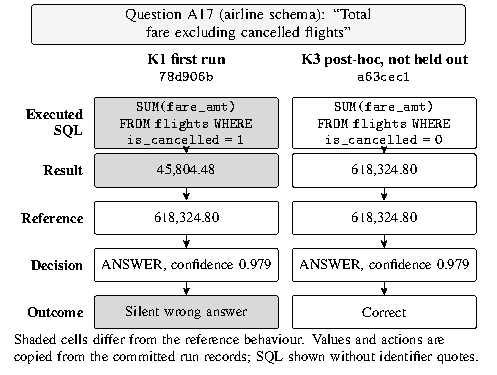
\includegraphics[width=\columnwidth]{figures/fig_a17_trace.pdf}
\caption{Recorded execution trace for question A17 in the K1 first run (\texttt{78d906b}) and the post-hoc K3 run (\texttt{a63cec1}). SQL, values, decisions and outcomes are copied from the committed run records; K3 is not held out.}
\label{fig:a17}
\end{figure}

This case illustrates that a query can be valid and executable while reversing the meaning of a negated condition. Syntax checks alone would not identify the error.

\textbf{Case V07: Unsupported ratio request.} The question asked for total yield in tons per acre. The system returned separate sums for yield and acreage rather than calculating the requested ratio. The evaluation reference indicated that the system should have requested clarification. The answer was returned with a WARN action and an internal confidence score of approximately 0.979.

This case illustrates the difference between returning relevant measures and computing the requested analytical quantity. The presence of both yield and acreage in the result does not establish that the requested ratio has been calculated.

Both cases carried high internal confidence scores. In this evaluation, confidence alone did not reliably distinguish these incorrect outputs from correct answers.

\subsection{Unanswered Answerable Questions}

The K1 system left 11 answerable questions unanswered. Recorded failure patterns included unfamiliar foreign-key names, abbreviations, flags represented in related tables, negation phrasing, word-stem variants, and numeric comparisons.

Table~\ref{tab:errors} summarizes the observed failures, their status after the post-hoc changes, and the remaining limitations.

\begin{table*}[!t]
\caption{Error Analysis and Limitations}
\label{tab:errors}
\centering
\footnotesize
\setlength{\tabcolsep}{3pt}
\begin{tabular}{@{}>{\raggedright}p{0.15\textwidth}>{\raggedright}p{0.29\textwidth}>{\raggedright}p{0.25\textwidth}>{\raggedright\arraybackslash}p{0.26\textwidth}@{}}
\toprule
\textbf{Case or class} & \textbf{Observed} & \textbf{After post-hoc changes (K3, not held out)} & \textbf{Remaining limitation} \\
\midrule
A17: reversed exclusion & K1: \texttt{is\_\allowbreak{}cancelled = 1}; 45,804.48 vs.\ reference 618,324.80; ANSWER at 0.979; silent wrong & Correct (\texttt{is\_\allowbreak{}cancelled = 0}); rule \texttt{polarity\_\allowbreak{}inverted} added & Fix informed by the K1 failure; not tested on held-out questions \\
V07: ``per acre'' ratio & K1: two separate sums; WARN at 0.979; silent wrong & CLARIFY at 0.30; rule \texttt{ratio\_\allowbreak{}unsupported} added & Ratios of two measures are clarified, not computed \\
Unanswered answerable questions & K1: 11/54; question families: numeric filter 2, abbreviation 2; undetected foreign key, time, nulls, related flag, fan-out, negation, flag 1 each & 5/54; families: abbreviation, flag, numeric filter, single value, undetected foreign key 1 each & Coverage is traded for conservative clarification \\
Historical D01, D02 & \texttt{3c843de}: reference SQL returns only the July total; disagreements not adjudicated & Not applicable & Requires semantic reference annotation \\
Verifier exceptions & Fail-open at \texttt{78d906b} and \texttt{a63cec1} & Fail-open & Fail-closed from \texttt{b11793b}, included in the R7 revision; no verifier exception occurred in any R7 run \\
Scope of the semantic layer & Not applied to the demo dataset or to intents other than direct KPI, breakdown, top-$N$, trend & \texttt{ratio} intent kind added & Other intents rely on the earlier checks only (R7 case IN14 is a distinct count) \\
Unsupported patterns & Ratios of measures, period-over-period with dimensions, share of total over joins, many-to-many grouping, anti-joins, non-ISO dates, undeclared foreign keys, non-SQLite engines, non-English questions & Unchanged & Outside the current rules; undeclared foreign keys are inferred only with name or key-suffix evidence (R7 revision) \\
\midrule
R7 wrong values (3 of 74 answerable) & RI12: ``not paid in cash'' kept only cash trips (204 vs.\ 1,039); IN04: ``claimed amount'' not bound, rows counted per adjuster at confidence 0.996; IN14: correct distinct count with an unrequested sum column appended & R7 revision frozen; no changes after the run & Negated value filters, fallback to a row count, and extra columns are not covered by the current rules \\
R7 answers to clarification items (4 of 31) & HO08: one of two date columns chosen; HO21: ``doing best'' resolved to a booking count; RI24: ``tip rate'' answered as a sum; IN28: ``average claim'' (flagged borderline by its author) & Frozen & Vague metrics and ``rate'' wording are not modelled \\
R7 unanswered (57 of 74 answerable) & Unbound measure paraphrases 20; ordinary words flagged by the unexplained-word check 11; unbound dimension words or negative-existence phrasing 11; unused column words 7; unused numbers 3; other 5 & Frozen & Lexical grounding on unfamiliar wording; the same checks prevent most wrong answers (Section~\ref{sec:ablation}) \\
\bottomrule
\end{tabular}
\end{table*}

These cases indicate that conservative handling can limit coverage even when a query may be answerable with the available data. The result highlights two separate objectives for future work: preventing unsupported answers and reducing unnecessary clarification.

A useful semantic validation system must address both. Excessive clarification can make a system less useful, while overly permissive query generation can produce plausible but incorrect results. Reporting only the number of correct answers would not adequately describe this trade-off.

\subsection{Post-Hoc K3 Results}

After the K1 failure cases had been inspected, the tuned K3 configuration achieved the following results on the same 66-question set:

\begin{itemize}
\tightlist
\item
  49 correct answers among 54 answerable questions;
\item
  49 answered questions among 54 answerable questions;
\item
  zero observed silent wrong answers among the 66 questions;
\item
  12 correct clarifications among 12 clarification-labelled cases; and
\item
  median and 95th-percentile latency of 15 ms and 43 ms.
\end{itemize}

Table~\ref{tab:results} and Fig.~\ref{fig:k1k3} compare the K1 and K3 results.

\begin{figure}[!t]
\centering
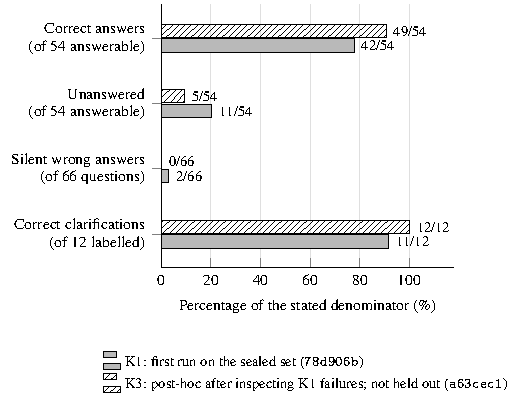
\includegraphics[width=\columnwidth]{figures/fig_k1_k3.pdf}
\caption{Round 6 K1 first run (\texttt{78d906b}) versus K3 post-hoc run (\texttt{a63cec1}) on the same 66 sealed questions. Each bar is a percentage of the denominator stated on its label; counts are printed beside the bars. K3 was measured after the K1 failures had been inspected and is not held out.}
\label{fig:k1k3}
\end{figure} K3 reflects development informed by observed failures. The result is evidence that targeted changes addressed the evaluated cases, but it is not an independent estimate of performance on unseen data. K1 therefore remains the primary first-run result, and K3 is not evidence that the semantic layer eliminates silent errors.

\subsection{Confidence Across First-Run Evaluation Sets}

The Round 6 calibration report also aggregates results from multiple first-run evaluation sets. In the pooled report, 23 silent wrong answers were recorded among 177 outputs with confidence at least 0.9. This aggregate spans multiple question sets and is not the K1-only rate.

The pooled result reinforces the K1 observation that high confidence does not guarantee correctness. Its scope is pooled across sets, and it is not a substitute for a K1-specific calibration analysis.

A complete calibration study would require an explicitly defined evaluation population, stable semantic labels, documented treatment of clarification and abstention, and a consistent calculation procedure. The current evidence is sufficient to motivate that analysis but does not establish that the confidence score is calibrated.

\subsection{Round 7 First-Run Results}

Table~\ref{tab:results} lists the R7 first-run measures alongside the earlier experiments, and Table~\ref{tab:r7} adds intervals and the sensitivity analysis. The frozen build answered 17 of the 74 answerable questions, 14 of them correctly. It declined all 12 unsupported questions and 15 of the 19 questions labelled as requiring clarification. Of its 7 wrong answers, 3 are wrong values on answerable questions and 4 are answers to questions labelled as requiring clarification (Table~\ref{tab:errors}). Removing the 20 questions that the authoring agent had flagged as borderline gives 14 correct answers among 65 answerable questions and 5 wrong answers among 85 questions, so the conclusions do not depend on those labels.

Coverage is far lower than in K1 (42 of 54). The K1 questions were written in the same process as the implementation, whereas the R7 schemas and phrasing were new to it. The most frequent causes of an unnecessary clarification were measure phrases that the planner could not bind, such as ``amount claimed'', ``kilowatt-hours'' and ``room nights'', and ordinary words flagged by the unexplained-word check, such as ``break down'' and ``came from''.

\begin{table}[!t]
\caption{Round 7 First Run (Frozen Revision 38b60d1)}
\label{tab:r7}
\centering
\footnotesize
\setlength{\tabcolsep}{3pt}
\begin{tabular}{@{}>{\raggedright}p{0.50\columnwidth}>{\raggedleft\arraybackslash}p{0.44\columnwidth}@{}}
\toprule
\textbf{Measure} & \textbf{Value [95\% Wilson interval]} \\
\midrule
Correct / answerable & 14/74 = 18.9\% [11.6, 29.3] \\
Correct / answered answerable & 14/17 = 82.4\% [59.0, 93.8] \\
Silent wrong / all questions & 7/105 = 6.7\% [3.3, 13.1] \\
Declined: clarification / unsupported & 15/19 / 12/12 \\
Without 20 borderline items & 14/65 correct; 5/85 wrong \\
Confidence of answers (min) & 0.979 \\
ECE, answered items, 5 bins & 0.32 \\
AUROC, correct vs.\ wrong answers & 0.67 \\
Latency, median / p95 & 54 ms / 660 ms \\
\bottomrule
\end{tabular}
\end{table}

\subsection{Safeguard Ablation Results}
\label{sec:ablation}

Table~\ref{tab:ablation} and Fig.~\ref{fig:r7abl} summarize the ablations. Disabling all six safeguards (A7) raised wrong answers from 7 to 32 and correct answers from 14 to 17. Removing the mention-coverage and wording checks (A5) turned 21 of the full pipeline's clarifications into wrong answers and 3 into correct answers; used alone (B5), these checks prevented 24 of the 32 errors seen in A7 at the cost of 3 correct answers. The semantic layer used alone (B1) prevented 4 errors (RI19, EN09, EN10, EN12) without losing a correct answer; three of those are also caught by the coverage checks, so removing it from the full pipeline (A1) added one wrong answer (EN12). The confidence threshold rule, the result-consistency checks, the plan-to-SQL fidelity gate and the answer verifier changed no outcome in any configuration. This does not show that they are ineffective in general, since regression tests exercise them on constructed failures, but this question set did not trigger them. Every executed answer scored at least 0.979, so the 0.70 and 0.40 thresholds never applied.

\begin{table}[!t]
\caption{Round 7 Safeguard Ablation (105 Questions; 74 Answerable)}
\label{tab:ablation}
\centering
\footnotesize
\setlength{\tabcolsep}{2.5pt}
\begin{tabular}{@{}>{\raggedright}p{0.44\columnwidth}>{\centering}p{0.12\columnwidth}>{\centering}p{0.13\columnwidth}>{\centering}p{0.11\columnwidth}>{\centering\arraybackslash}p{0.14\columnwidth}@{}}
\toprule
\textbf{Configuration} & \textbf{Correct} & \textbf{Answered} & \textbf{Wrong} & \textbf{Unnec.\ clarif.} \\
\midrule
A0 full pipeline & 14 & 17 & 7 & 57 \\
A1 without semantic layer & 14 & 18 & 8 & 56 \\
A2 without confidence threshold & 14 & 17 & 7 & 57 \\
A3 without result consistency & 14 & 17 & 7 & 57 \\
A4 without plan fidelity gate & 14 & 17 & 7 & 57 \\
A5 without coverage + wording & 17 & 38 & 28 & 36 \\
A6 without answer verifier & 14 & 17 & 7 & 57 \\
A7 all six removed & 17 & 41 & 32 & 33 \\
B1 only semantic layer & 17 & 38 & 28 & 36 \\
B5 only coverage + wording & 14 & 18 & 8 & 56 \\
\bottomrule
\end{tabular}

\vspace{3pt}
\parbox{\columnwidth}{\scriptsize Correct and Answered: of 74 answerable. Wrong: of 105 questions. B2, B3, B4 and B6 equal A7. A5 removes two checks in one stage and is confounded between them.}
\end{table}

\begin{figure}[!t]
\centering
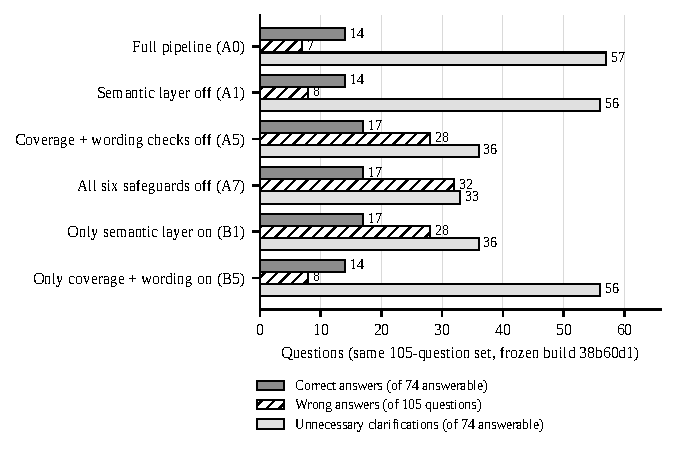
\includegraphics[width=\columnwidth]{figures/fig_r7_ablation.pdf}
\caption{Round 7 ablation on the frozen revision \texttt{38b60d1}: correct answers, wrong answers and unnecessary clarifications for configurations that change at least one outcome. A2, A3, A4 and A6 equal A0.}
\label{fig:r7abl}
\end{figure}

\subsection{Confidence on Round 7}

All 21 answers of the full pipeline, and all 49 answers with the safeguards disabled, scored between 0.979 and 1.0; every wrong answer was therefore a high-confidence error. Accuracy among answered questions was 0.67 in A0 and 0.35 in A7, against a mean score near 0.985, giving expected calibration errors of 0.32 and 0.64 \cite{naeini2015bbq}. The area under the ROC curve for separating correct from wrong answers was 0.67 and 0.69. This weak separation follows answer shape rather than correctness: plain scalar answers receive 0.979, while breakdowns that reconcile with their totals receive 0.99--1.0, and most wrong answers were scalars. A higher threshold could trade coverage for risk, but such an operating point would have to be chosen on held-out data. The protection measured in Section~\ref{sec:ablation} comes from checks that override the decision, not from the score.

\subsection{Round 8: Revised Build on Revealed and Blind Questions}

On the revealed R7 questions the revised build answers 63 of 74 answerable questions correctly and gives 2 wrong answers among 105, against 14 and 7 in the R7 first run; 49 correct answers were gained and none lost. These questions informed the changes, so this is a post-hoc development result. On the blind R8 set the same frozen build answered 11 of 73 answerable questions, 5 correctly (6.8\%, 95\% CI 3.0--15.1\%), refused 29 of 33 questions that required clarification or were unsupported, and gave 10 wrong answers among 106 questions (9.4\%, 95\% CI 5.2--16.5\%), see Table~\ref{tab:r8}. R7 and R8 use different questions, so the two first runs are not a paired comparison; but the revised build shows no improvement on unseen data, and the post-hoc gain must be read as fitting to the questions that motivated it. The R8 wrong answers include new classes: a time-unit word (``monthly rent'') read as a trend over a numeric column at confidence 1.0, an inverted date-state condition (``ever signed''), a product of two columns returned as two sums, and vague requests (``big orders'', ``top-paying tenants'') answered with a default metric.

\begin{table}[!t]
\caption{Round 8: Revised Build (da925ad) on Revealed (Post-Hoc) and Blind Questions}
\label{tab:r8}
\centering
\footnotesize
\setlength{\tabcolsep}{3pt}
\begin{tabular}{@{}>{\raggedright}p{0.40\columnwidth}>{\centering}p{0.26\columnwidth}>{\centering\arraybackslash}p{0.26\columnwidth}@{}}
\toprule
 & \textbf{R7 set, post-hoc} & \textbf{R8 blind, first run} \\
\midrule
Questions (answerable / other) & 105 (74 / 31) & 106 (73 / 33) \\
Correct / answerable & 63/74 & 5/73 \\
Answered / answerable & 64/74 & 11/73 \\
Wrong answers / all & 2/105 & 10/106 \\
Appropriate refusals & 30/31 & 29/33 \\
All safeguards off: correct / wrong & 64 / 9 & 9 / 35 \\
Latency, median / p95 (ms) & 214 / 796 & 319 / 1,741 \\
\bottomrule
\end{tabular}

\vspace{3pt}
\parbox{\columnwidth}{\scriptsize The R7 column is post-hoc (the questions guided the changes) and is not held out. R8 questions are agent-generated, not human-adjudicated.}
\end{table}

The ablations on R8 repeat the R7 pattern. Disabling all six safeguards gives 9 correct and 35 wrong answers. Used alone, the mention-coverage and wording checks prevent 23 of those 35 errors at the cost of 4 correct answers, the semantic layer prevents 4, and the plan-to-SQL fidelity gate prevents 2; the confidence threshold, the result-consistency checks and the answer verifier change no outcome. On R8 every answer scored at least 0.835 and 9 of the 10 wrong answers scored at least 0.9; the area under the ROC curve for separating correct from wrong answers was 0.45 (0.48 with the safeguards disabled), no better than chance, and the expected calibration error was 0.64.

\section{Discussion}

The experiments provide several observations relevant to the design of conversational business intelligence systems.

First, successful SQL execution is not sufficient evidence that an analytical request has been answered correctly. The historical benchmark demonstrated high execution success, but two reference-query disagreements remained unresolved because the intended diagnostic comparison was not fully specified. The K1 semantic-layer evaluation provided more concrete examples: a reversed exclusion filter and an unsupported ratio request both resulted in incorrect high-confidence answers.

Second, semantic checks need to examine the meaning of analytical operations, not only the validity of the SQL statement or the existence of referenced columns. Negation, ratios, temporal interpretation, join relationships, and aggregation grain are all possible sources of semantic mismatch. The current checks cover selected examples of these issues, but the K1 errors show that their coverage is incomplete.

Third, confidence should be treated as one input to response selection rather than as a substitute for semantic verification. The two K1 silent wrong answers had mean confidence close to 0.98, comparable to the confidence recorded for correct answers. This observation does not mean that confidence estimates are useless in every setting. It means that their reliability must be established empirically and that high scores should not override explicit semantic violations.

Fourth, answer coverage and error risk must be evaluated jointly. K1 left 11 answerable questions unanswered, including questions affected by abbreviations and schema relations. These cases show that conservative handling can avoid some unsupported responses while also preventing valid questions from being answered. Future evaluation should report coverage, correctness, silent wrong answers, and clarification quality together.

Fifth, R7 shows how strongly the earlier first-run results depended on schemas and wording written in the same process as the implementation. On new schemas and phrasing, coverage fell to 17 of 74 answerable questions while wrong answers stayed at 7 of 105. The ablation shows that this caution is not incidental: the checks that compare the question's words with the executed query prevented 24 of the 32 errors seen without safeguards, and the same checks account for most unnecessary clarifications. Improving grounding without weakening those checks is therefore the main engineering problem identified by this study. Round 8 shows how hard that problem is: grounding changes derived from inspected failures fixed those failures but did not raise accuracy on new schemas and wording, while the checks again prevented most of the errors that the planner would otherwise have returned.

Finally, the difference between K1 and K3 illustrates the importance of separating first-run and post-hoc results. Targeted fixes can improve performance on known failure cases, but those improvements do not provide an unbiased estimate of generalization. A stronger evaluation should freeze the implementation before independent question sets are revealed and should reserve an untouched set for final testing.

\section{Limitations}

This study has several limitations.

\textbf{Synthetic datasets and limited scale.} The experiments use relatively small, synthetic datasets. The historical and Round 6 questions were written by the authors; the R7 questions were generated by an AI agent of the same model family as the development agent, under instructions not to read the implementation, and no human adjudicated their labels. R7 is therefore provisional evidence, and its intervals are wide. The results do not establish performance on production enterprise data, broader user populations, or naturally occurring business questions.

\textbf{Reference ambiguity.} Reference SQL does not always fully specify the intended analytical meaning of a question. This limitation is particularly relevant to diagnostic questions involving explanations for changes in metrics. Future evaluation should include semantic reference annotations and independent adjudication of ambiguous cases.

\textbf{Database coverage.} All reported database experiments use SQLite. Performance and correctness on PostgreSQL or other database engines have not been established by these experiments.

\textbf{Partial semantic coverage.} The semantic layer is rule-based and does not cover every possible query pattern. Known limitations include ratios of measures, period-over-period comparisons combined with dimensions, share-of-total calculations over joins, many-to-many grouping, anti-joins, non-ISO date formats, and foreign-key relationships that are not declared or inferable. Heuristic synonyms and word stems may also over-trigger or fail to identify intended concepts; in R7 they caused most of the 57 unnecessary clarifications. R7 also exposed error classes that the rules do not cover: a negated value filter applied with the wrong polarity, an unbound measure phrase that fell back to a row count, an unrequested extra column, and ``rate'' wording answered as a sum. The layer is not applied to the built-in demo dataset or to intents other than direct KPI, breakdown, top-$N$, trend and, from revision \texttt{a63cec1}, the \texttt{ratio} intent kind (Fig.~\ref{fig:semflow}).

\textbf{Post-hoc evaluation.} The 63 of 74 correct answers of the revised build on the R7 questions are post-hoc; the blind R8 result (5 of 73) is the relevant estimate for that build. K3 was tuned after K1 failure cases had been inspected. The K3 results are therefore not independent held-out evidence and should not be used as the main estimate of generalization.

\textbf{Confidence calibration.} The observed high-confidence errors show that the current confidence score is not a sufficient guarantee of correctness. In R7 every answer scored at least 0.979 and the expected calibration error was 0.32. The reported values do not establish calibrated probabilities, and the pooled calibration report covers several different evaluation sets.

\textbf{Ablation scope.} Four of the six safeguards changed no R7 outcome; their value is not demonstrated by this evaluation. The coverage and wording checks were ablated together and are not separated.

\textbf{Latency and deployment.} Latency measurements come from local runs. They do not establish performance under production networking, concurrent workloads, or deployment-level conditions.

\textbf{External comparison.} The study does not provide a controlled comparison against established text-to-SQL baselines on the same question set, schemas, and execution protocol. The results therefore do not support a claim of superiority over existing systems. For R7, no language-model access or downloadable baseline was available in the evaluation environment; the configuration with all safeguards disabled is an internal reference, not an external baseline.

\section{Conclusion and Future Work}

This paper presented InsightFlow AI, an inspectable conversational business intelligence prototype combining query planning, confidence-aware response selection, evidence recording, and a rule-based semantic correctness layer.

The historical sales benchmark showed that the earlier pipeline executed SQL for all 17 answerable questions and agreed with reference SQL on 15 of those cases. However, the two disagreements were not independently adjudicated for intended semantics, and the five historical configurations produced identical outcomes on the benchmark.

In the separate Round 6 first-run evaluation, the semantic-layer implementation produced 42 correct answers among 54 answerable questions, left 11 answerable questions unanswered, and generated two silent wrong answers among 66 questions. Both silent errors carried internal confidence scores near 0.98. These findings show that semantic errors remain possible even when a system exposes confidence and performs explicit checks.

In the Round 7 first run on four new agent-authored schemas, a later frozen revision answered 14 of 74 answerable questions correctly, declined 27 of 31 questions that required clarification or were unsupported, and gave 7 wrong answers among 105 questions, against 32 with its post-generation safeguards disabled. The checks comparing the question with the executed query produced most of this reduction; the confidence score did not separate correct from wrong answers.

A revised build that fixed the inspected R7 failures answered 63 of 74 of those questions correctly but only 5 of 73 on a new blind set (R8), with 10 wrong answers among 106; its improvements did not generalize, and on R8 its confidence score was no better than chance at separating correct from wrong answers.

The post-hoc K3 results improved on the evaluated cases, but they should be interpreted as targeted engineering results rather than independent evidence of generalization. The overall findings support further investigation of inspectable semantic validation, while underscoring the need to evaluate correctness, coverage, clarification behaviour, and confidence together.

Future work should focus on independently authored and sealed question sets, semantic reference annotations reviewed by independent evaluators, broader schema and database coverage, and controlled comparisons with suitable baseline systems. Evaluation should also examine whether the semantic layer improves the balance between useful answer coverage and the risk of silent wrong answers on unseen data.

The current results do not establish that semantic errors have been eliminated or that InsightFlow AI is superior to existing text-to-SQL systems. They provide a reproducible starting point for examining how explicit semantic checks can support more inspectable conversational analytics.

\section*{Reproducibility Statement}

The project source code and evaluation artifacts are maintained at:

\url{https://github.com/jagan1344/insightflow-ai}

The historical sales benchmark is associated with commit \texttt{3c843de88c\allowbreak{}a0b6266974\allowbreak{}9b217aaef0\allowbreak{}00e3e6363e}. The Round 6 first-run implementation was frozen at commit \texttt{78d906b} before the sealed questions were inspected. The K3 results were obtained after inspection and tuning and are reported separately.

The Round 6 seal file, \texttt{evaluation/\allowbreak{}v3/\allowbreak{}FINAL6\_SEAL.txt}, records SHA-256 digests for the sealed question and fixture files. Revision \texttt{b11793b}, committed after both Round 6 runs, makes the semantic verifier fail closed on internal errors; at that revision the backend regression suite passed (495 tests, 3 warnings). These tests check implementation behavior; they are not an accuracy benchmark, and no Round 6 results are reported for that revision.

The Round 7 build was frozen at revision \texttt{38b60d1} after 526 regression tests passed. The R7 questions, reference results, databases and protocol are in \texttt{evaluation/\allowbreak{}v5\_provisional/} and \texttt{research\_\allowbreak{}improvement/\allowbreak{}eval/}; the SHA-256 manifest \texttt{V5\_MANIFEST.sha256} was committed before the first run, and the raw first-run output (\texttt{v5\_A0\_first\_run.json}) was committed before it was scored. Ablation runs, the confidence analysis and a script that recomputes every reported R7 figure are in \texttt{research\_\allowbreak{}improvement/}. The revised build is frozen at \texttt{da925ad}; the R8 questions are in \texttt{evaluation/\allowbreak{}v6\_blind/}, and their protocol, manifest, raw first run (committed before scoring), ablations and analysis are in \texttt{research\_\allowbreak{}improvement/\allowbreak{}accuracy\_\allowbreak{}improvement/}.

\begin{thebibliography}{00}
\bibitem{zhong2017seq2sql} V. Zhong, C. Xiong, and R. Socher, ``Seq2SQL: Generating structured queries from natural language using reinforcement learning,'' 2017, arXiv:1709.00103.
\bibitem{yu2018spider} T. Yu \emph{et al.}, ``Spider: A large-scale human-labeled dataset for complex and cross-domain semantic parsing and text-to-SQL task,'' in \emph{Proc. Conf. Empirical Methods Natural Lang. Process. (EMNLP)}, 2018, pp. 3911--3921.
% [3] The source draft's track designation ("Datasets and Benchmarks") could not be verified; add it only if confirmed.
\bibitem{li2023bird} J. Li \emph{et al.}, ``Can LLM already serve as a database interface? A big bench for large-scale database grounded text-to-SQLs,'' in \emph{Adv. Neural Inf. Process. Syst. (NeurIPS)}, 2023.
\bibitem{lei2025spider2} F. Lei \emph{et al.}, ``Spider 2.0: Evaluating language models on real-world enterprise text-to-SQL workflows,'' in \emph{Proc. Int. Conf. Learn. Represent. (ICLR)}, 2025, arXiv:2411.07763.
\bibitem{geifman2017selective} Y. Geifman and R. El-Yaniv, ``Selective classification for deep neural networks,'' in \emph{Adv. Neural Inf. Process. Syst.}, vol. 30, 2017, pp. 4878--4887.
\bibitem{naeini2015bbq} M. P. Naeini, G. F. Cooper, and M. Hauskrecht, ``Obtaining well calibrated probabilities using Bayesian binning,'' in \emph{Proc. AAAI Conf. Artif. Intell.}, 2015, pp. 2901--2907.
\bibitem{yao2023react} S. Yao \emph{et al.}, ``ReAct: Synergizing reasoning and acting in language models,'' in \emph{Proc. Int. Conf. Learn. Represent. (ICLR)}, 2023.
% [8] Add an access date; the specification revision implemented by the MCP servers is not established.
\bibitem{mcp} Model Context Protocol, ``Specification.'' [Online]. Available: \url{https://modelcontextprotocol.io/}
\bibitem{insightflowrepo} InsightFlow AI project repository, ``Source code and evaluation artifacts.'' Accessed: Oct. 25, 2026. [Online]. Available: \url{https://github.com/jagan1344/insightflow-ai}
\end{thebibliography}

\end{document}
